\documentclass[10pt,a4paper]{article}
\usepackage[T1]{fontenc}
\usepackage[utf8]{inputenc}
\usepackage{mathptmx}
\usepackage[left=2cm,right=2cm,top=1.6cm,bottom=1.6cm]{geometry}
\usepackage{amsmath,amssymb}
\usepackage{graphicx}
\usepackage{booktabs}
\usepackage{float}
\usepackage{array}
\usepackage{microtype}
\usepackage[font=small,labelfont=bf,skip=4pt]{caption}
\usepackage{titlesec}
\usepackage{enumitem}
\usepackage{xcolor}
\usepackage{listings}
\usepackage[hidelinks]{hyperref}

\titlespacing*{\section}{0pt}{6pt plus 2pt minus 1pt}{3pt}
\titlespacing*{\subsection}{0pt}{5pt plus 1pt minus 1pt}{2pt}
\titleformat{\section}{\normalfont\large\bfseries}{\thesection}{0.6em}{}
\titleformat{\subsection}{\normalfont\normalsize\bfseries}{\thesubsection}{0.6em}{}
\setlist[itemize]{topsep=2pt,itemsep=1pt,parsep=0pt,leftmargin=1.2em}
\setlist[enumerate]{topsep=2pt,itemsep=1pt,parsep=0pt,leftmargin=1.4em}
\setlength{\abovedisplayskip}{4pt}
\setlength{\belowdisplayskip}{4pt}
\setlength{\textfloatsep}{8pt}
\renewcommand{\arraystretch}{1.05}
\linespread{0.97}\selectfont

\lstset{basicstyle=\ttfamily\scriptsize, columns=fullflexible, keepspaces=true,
        breaklines=true, frame=lines, numbers=left, numberstyle=\tiny\color{gray},
        commentstyle=\color{gray}, stringstyle=\color{teal!70!black},
        keywordstyle=\bfseries, showstringspaces=false, upquote=true}

\title{\vspace{-1.2cm}\bfseries The Clarke \& Wright Savings Heuristic for the\\
Capacitated Vehicle Routing Problem: Sequential and Parallel Versions}
\author{Heuristic Algorithms in Transport and Finance --- Master's course assignment \\
    Javier Salvatierra \\
    Jesús Inurria
}
\date{September 2026}

\begin{document}
\maketitle
\vspace{-0.8cm}

\begin{abstract}
\noindent\small
The Capacitated Vehicle Routing Problem (CVRP) asks for a set of minimum-cost routes that start and end
at a depot, visit every customer exactly once and never exceed the capacity of a vehicle. We describe
the savings heuristic of Clarke and Wright (CWS), implement its sequential and parallel versions in
Python --- the parallel one also in C++ --- and test them on the 33 classical benchmark instances used
by Juan et al.~(2011). The parallel CWS reproduces the CWS cost reported by Juan et al.\ in 27 of the 33
instances (all 33 with tied savings ordered the other way round), $4.91\,\%$ above the best-known
solutions on average; the sequential one is $11.6\,\%$ worse. Both take milliseconds in Python, and
the C++ port returns the same solutions in 13\,\textmu s--1.4\,ms.
\end{abstract}

\section{Introduction}

The Vehicle Routing Problem (VRP) generalises the
Travelling Salesman Problem (TSP). In the TSP a single traveller visits every city once along the
shortest closed tour. In the VRP a \emph{fleet} of vehicles leaves a common depot, every customer is
visited by exactly one vehicle and every vehicle returns to the depot: one must decide how the customers
are split into routes and in which order each route visits them, minimising the total distance.

In the \emph{capacitated} version (CVRP) the vehicles carry goods: each vehicle has capacity $Q$ and each
customer $i$ consumes a demand $q_i$ from it, so the total demand served by a route cannot exceed $Q$.
The CVRP contains the TSP as the special case of a single vehicle with unlimited capacity, and it is
therefore NP-hard, which has motivated many heuristics that find near-optimal solutions quickly. The savings heuristic of Clarke
and Wright~\cite{cw1964} (CWS) is probably the most cited of them~\cite{juan2011}: it is simple, has no
parameters, and gives solutions typically 5--10\,\% above the best known in milliseconds~\cite{slides}.

We test the heuristic on the 33 classical CVRP instances selected by Juan et al.~\cite{juan2011}, which
come from six classical families (\texttt{A}, \texttt{B}, \texttt{E}, \texttt{F}, \texttt{M} and
\texttt{P}), with random, clustered and real-world customer layouts. An instance named \texttt{A-n32-k5} has $n=32$
nodes (the depot and 31 customers) and a best-known solution with $k=5$ vehicles; sizes range from 22 to
135 nodes. The depot is central in some instances and in a corner in others. Each file gives the coordinates and the demand of every node, with the
depot translated to the origin; the capacity $Q$ and the reference costs are taken from Table~1
of~\cite{juan2011}. Below we state the model, describe the CWS and our implementation, and compare the results with
that table.

\section{Problem formulation and savings}
\label{sec:model}

Let node $0$ be the depot and $N=\{1,\dots,n-1\}$ the set of customers. Every customer $i$ has a demand
$0<q_i\le Q$, and $c(i,j)=c(j,i)$ is the Euclidean distance between nodes $i$ and $j$, not rounded. The
fleet consists of identical vehicles of capacity $Q$; the CWS does not fix their number, so a solution
may use more vehicles than the $k$ of the instance name. A solution is a set of routes $R_1,\dots,R_m$,
each an ordered sequence of customers travelled as $0\to R_r\to0$, and the CVRP reads
\begin{equation}
\min\ \sum_{r=1}^{m} c(R_r)
\qquad\text{s.t.}\qquad
R_1\cup\dots\cup R_m = N,\quad R_r\cap R_s=\emptyset\ (r\neq s),\qquad
\sum_{i\in R_r} q_i\le Q\quad (r=1,\dots,m),
\label{eq:cvrp}
\end{equation}
where $c(R_r)$ is the length of the closed tour of route $r$: every customer is visited exactly once and
no route is overloaded.

Serving every customer with its own vehicle, $0\to i\to0$, costs $2\,c(0,i)$ per customer (there and
back), $2\sum_{i\in N}c(0,i)$ in total. If two customers $i$ and $j$ are instead served consecutively by the same vehicle,
the return $i\to0$ and the departure $0\to j$ are replaced by the direct edge $i\to j$, which saves
\begin{equation}
s(i,j) = c(0,i) + c(0,j) - c(i,j).
\label{eq:savings}
\end{equation}
By the triangle inequality, $c(i,j)\le c(i,0)+c(0,j)$, so $s(i,j)\ge0$: going directly from one customer
to the next is never longer than going back to the depot in between. Savings are largest for customers
that are close to each other and far from the depot.

\section{The Clarke and Wright savings heuristic}
\label{sec:cws}

Clarke and Wright~\cite{cw1964} build a solution by starting from the dummy solution above and merging
routes along the edges with the largest savings, as long as the constraints of~\eqref{eq:cvrp} hold.

\subsection{Dummy solution}

The initial solution assigns one vehicle to each customer. It is feasible because $q_i\le Q$, every
customer is visited once and receives its demand $q_i$, and it has the largest possible cost. The savings
$s(i,j)$ of all $\binom{n-1}{2}$ pairs of customers are computed and sorted in decreasing order into the
\emph{savings list}.

\subsection{Improving the dummy solution by merging routes}

The heuristic walks down the savings list. For an edge $(i,j)$, the route that contains $i$ and the route
that contains $j$ are merged into one route that goes through $i\to j$ if three conditions hold:
\begin{enumerate}
\item \textbf{Different routes.} If $i$ and $j$ were already on the same route, the new edge would close
a cycle that does not visit the depot.
\item \textbf{Both nodes are exterior}, i.e.\ adjacent to the depot (first or last customer of their
route). An interior customer already has two neighbours and cannot receive a third one.
\item \textbf{Capacity.} The joint load of the two routes does not exceed $Q$.
\end{enumerate}
A merge replaces $(i,0)$ and $(0,j)$ by $(i,j)$, so the cost drops by exactly $s(i,j)\ge0$; taking the
edges in decreasing order of saving makes the heuristic greedy. There are two
classical ways of walking the list~\cite{cw1964,juan2011}:
\begin{itemize}
\item \textbf{Parallel CWS.} The list is walked once, and \emph{any} two routes are merged whenever the
conditions hold, so all routes grow at the same time. This is the version used by Juan et al.\ because it
usually gives better results~\cite{juan2011}.
\item \textbf{Sequential CWS.} One route is grown at a time: it is extended with the best feasible edge
that touches one of its two ends until none is left, then it is closed and the next route is started.
\end{itemize}
In both versions an edge that fails the conditions can be discarded for good: routes only grow, so a
node that became interior stays interior, two nodes on the same route stay together and loads only
increase.

\section{Implementation}
\label{sec:impl}

Juan et al.~\cite{juan2011} build SR-GCWS-CS on top of the CWS: a multi-start method that picks the next
edge at random (geometric distribution) from the top of the list, caches the best order of every route
and splits the plane into sub-problems. We implement only the classic, deterministic CWS, lines 1--2 of
their Figure~4 (savings list and CWS solution); our loop has the structure of their Figure~5 but always
takes the first edge. The reference is thus the column \emph{CWS Sol.} of their Table~1, not \emph{Our
Best Sol.}

The code (Appendix~\ref{app:code}) is a Python~3.14 module, \texttt{vrp.py}, built on NumPy, plus a
C++ port of the parallel version. Distances are computed once
as an $n\times n$ matrix, and the savings list is sorted with a \emph{stable} sort, so edges with equal
saving keep their generation order $(i,j)$ with $i<j$, as in the course code~\cite{slides}.

\subsection{Common objects: the dummy solution}

Both versions start from \texttt{construct\_initial\_sol}, which builds three objects kept up to date
by the algorithm: \texttt{routes}, a dictionary \emph{route index $\to$ list of customers} (the depot at
both ends is implicit; initially route $i$ is \texttt{[i]}); \texttt{route\_of}, the route index of
every node, so that the route of a customer is found in $O(1)$; and \texttt{load}, the demand carried by
each route, so that the capacity check is $O(1)$.
The conditions of Section~\ref{sec:cws} are checked by \texttt{check\_merging\_conditions}. A merge
(\texttt{merge\_routes\_using\_edge}) reverses the routes if needed so that the first one ends at $i$ and
the second one starts at $j$, concatenates them, relabels the customers of the second route in
\texttt{route\_of} and adds up the loads.

\subsection{Sequential version}

\texttt{sequential\_cws} seeds a route with the first feasible edge of the list, then scans the list again
from the top for the first feasible edge with one end on the current route, merges, and repeats. When no
edge can extend the route, the route is closed and a new one is seeded; the heuristic stops when no
feasible edge is left. Edges that touch the current route and fail the conditions are deleted; edges
that do not touch it are kept for the routes still to come.

\subsection{Parallel version in Python and C++}

\texttt{parallel\_cws} reuses the same building blocks and differs only in the way the list is walked:
each edge is tried exactly once, in decreasing order of saving, and merges the routes of its two nodes,
whichever they are, if the conditions hold. The C++ file \texttt{cws.cpp} ports it function by function
(\texttt{std::stable\_sort} for the list) and is compiled with Clang through Zig (\texttt{zig c++ -O2
-ffp-contract=off}). Disabling fused multiply--add keeps every floating-point operation identical to
NumPy, so savings, ties and costs match bit for bit: the 33 solutions are the same.

\section{Computational results}
\label{sec:res}

Table~\ref{tab:results} compares both versions with Table~1 of~\cite{juan2011}, with
$\text{gap}=100\,(\text{cost}-\text{ref})/\text{ref}$. Times cover the savings list and the construction: one run in
Python, the mean of repeated runs over at least 0.1\,s in C++.

\begin{table}[!t]
\centering
\caption{Sequential and parallel CWS. \emph{BKS} (real distances) and \emph{JORS CWS} from Table~1
of~\cite{juan2011}; routes in bold exceed $k$; times of the parallel CWS.}
\label{tab:results}
\scriptsize
\setlength{\tabcolsep}{4pt}
\begin{tabular}{@{}lrrrrrrrrrrr@{}}
\toprule
 & & & JORS & Seq. & Seq.\ vs & Par.\ & Par.\ vs & Par.\ vs & Par. & Python & C++ \\
Instance & $Q$ & BKS & CWS & cost & JORS (\%) & cost & JORS (\%) & BKS (\%) & routes & (ms) & (\textmu s) \\
\midrule
\texttt{A-n32-k5} & 100 & 787.81 & 843.69 & 907.11 & 7.52 & 843.69 & 0.00 & 7.09 & 5 & 1.23 & 38 \\
\texttt{A-n38-k5} & 100 & 734.18 & 768.14 & 834.26 & 8.61 & 768.13 & 0.00 & 4.62 & \textbf{6} & 1.61 & 38 \\
\texttt{A-n45-k7} & 100 & 1\,147.28 & 1\,199.98 & 1\,251.38 & 4.28 & 1\,199.98 & 0.00 & 4.59 & 7 & 2.20 & 60 \\
\texttt{A-n55-k9} & 100 & 1\,074.46 & 1\,099.84 & 1\,290.89 & 17.37 & 1\,099.84 & 0.00 & 2.36 & 9 & 3.12 & 125 \\
\texttt{A-n60-k9} & 100 & 1\,355.80 & 1\,421.88 & 1\,572.97 & 10.63 & 1\,421.88 & 0.00 & 4.87 & 9 & 3.66 & 158 \\
\texttt{A-n61-k9} & 100 & 1\,039.08 & 1\,102.23 & 1\,188.96 & 7.87 & 1\,102.23 & 0.00 & 6.08 & \textbf{10} & 3.95 & 165 \\
\texttt{A-n65-k9} & 100 & 1\,181.69 & 1\,239.42 & 1\,479.40 & 19.36 & 1\,239.42 & 0.00 & 4.89 & \textbf{10} & 4.25 & 234 \\
\texttt{A-n80-k10} & 100 & 1\,766.50 & 1\,860.94 & 1\,956.41 & 5.13 & 1\,860.94 & 0.00 & 5.35 & 10 & 6.23 & 422 \\
\texttt{B-n50-k7} & 100 & 744.78 & 748.80 & 849.34 & 13.43 & 748.80 & 0.00 & 0.54 & 7 & 2.59 & 82 \\
\texttt{B-n52-k7} & 100 & 750.08 & 764.90 & 839.92 & 9.81 & 764.90 & 0.00 & 1.98 & 7 & 2.72 & 104 \\
\texttt{B-n57-k9} & 100 & 1\,603.63 & 1\,653.42 & 1\,769.42 & 7.02 & 1\,653.42 & 0.00 & 3.11 & 9 & 3.37 & 136 \\
\texttt{B-n78-k10} & 100 & 1\,229.27 & 1\,264.56 & 1\,401.39 & 10.82 & 1\,264.56 & 0.00 & 2.87 & 10 & 5.96 & 376 \\
\texttt{E-n22-k4} & 6000 & 375.28 & 388.77 & 448.90 & 15.47 & 388.77 & 0.00 & 3.60 & 4 & 0.70 & 13 \\
\texttt{E-n30-k3} & 4500 & 535.80 & 534.45 & 611.05 & 14.33 & 534.45 & 0.00 & $-$0.25 & \textbf{4} & 1.03 & 33 \\
\texttt{E-n33-k4} & 8000 & 838.72 & 843.10 & 913.12 & 8.31 & 843.10 & 0.00 & 0.52 & 4 & 1.28 & 40 \\
\texttt{E-n51-k5} & 160 & 524.94 & 584.64 & 625.56 & 7.00 & 584.64 & 0.00 & 11.37 & \textbf{6} & 2.63 & 93 \\
\texttt{E-n76-k7} & 220 & 687.60 & 737.74 & 862.67 & 16.93 & 738.13 & 0.05 & 7.35 & 7 & 5.49 & 333 \\
\texttt{E-n76-k10} & 140 & 837.36 & 900.26 & 1\,005.25 & 11.66 & 907.39 & 0.79 & 8.36 & 10 & 5.64 & 337 \\
\texttt{E-n76-k14} & 100 & 1\,026.71 & 1\,073.43 & 1\,161.29 & 8.18 & 1\,054.60 & $-$1.75 & 2.72 & \textbf{15} & 6.01 & 363 \\
\texttt{F-n45-k4} & 2010 & 724.57 & 739.02 & 1\,003.09 & 35.73 & 739.02 & 0.00 & 1.99 & 4 & 2.08 & 71 \\
\texttt{F-n72-k4} & 30000 & 248.81 & 256.19 & 346.47 & 35.24 & 256.19 & 0.00 & 2.96 & \textbf{5} & 4.60 & 291 \\
\texttt{F-n135-k7} & 2210 & 1\,170.65 & 1\,219.32 & 1\,423.00 & 16.70 & 1\,219.32 & 0.00 & 4.16 & 7 & 15.95 & 1382 \\
\texttt{M-n101-k10} & 200 & 819.81 & 833.51 & 939.99 & 12.78 & 833.51 & 0.00 & 1.67 & 10 & 9.38 & 687 \\
\texttt{M-n121-k7} & 200 & 1\,045.16 & 1\,068.14 & 1\,291.33 & 20.90 & 1\,068.14 & 0.00 & 2.20 & 7 & 12.70 & 1011 \\
\texttt{P-n22-k8} & 3000 & 601.42 & 590.62 & 625.91 & 5.97 & 590.62 & 0.00 & $-$1.80 & \textbf{9} & 0.77 & 13 \\
\texttt{P-n40-k5} & 140 & 461.73 & 518.37 & 516.42 & $-$0.38 & 518.37 & 0.00 & 12.27 & 5 & 1.81 & 44 \\
\texttt{P-n50-k10} & 100 & 699.56 & 734.32 & 740.57 & 0.85 & 739.84 & 0.75 & 5.76 & \textbf{11} & 2.74 & 86 \\
\texttt{P-n55-k15} & 70 & 991.48 & 978.07 & 1\,036.48 & 5.97 & 978.07 & 0.00 & $-$1.35 & \textbf{17} & 3.56 & 113 \\
\texttt{P-n65-k10} & 130 & 796.67 & 851.67 & 938.51 & 10.20 & 851.67 & 0.00 & 6.90 & 10 & 4.33 & 196 \\
\texttt{P-n70-k10} & 135 & 830.02 & 896.86 & 957.87 & 6.80 & 896.86 & 0.00 & 8.05 & \textbf{11} & 4.86 & 261 \\
\texttt{P-n76-k4} & 350 & 598.22 & 689.13 & 724.08 & 5.07 & 688.34 & $-$0.11 & 15.07 & 4 & 5.15 & 301 \\
\texttt{P-n76-k5} & 280 & 635.04 & 698.51 & 793.37 & 13.58 & 709.38 & 1.56 & 11.71 & 5 & 5.28 & 298 \\
\texttt{P-n101-k4} & 400 & 692.28 & 765.38 & 843.70 & 10.23 & 765.38 & 0.00 & 10.56 & 4 & 8.72 & 692 \\
\midrule
\textbf{Mean} & & & & & \textbf{11.62} & & \textbf{0.04} & \textbf{4.91} & & 4.41 & 261 \\
\bottomrule
\end{tabular}
\end{table}

\begin{figure}[!htb]
\centering
\graphicspath{{../results/figures/}}
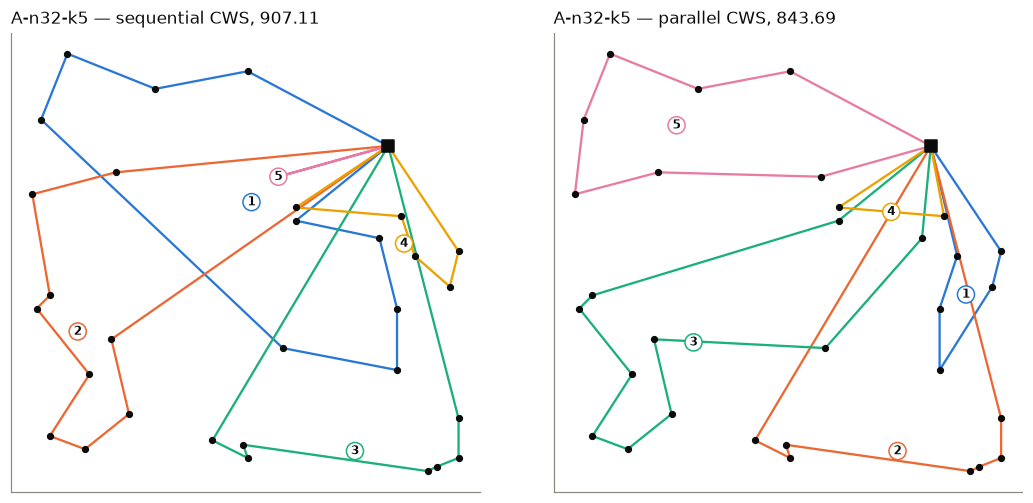
\includegraphics[width=0.46\textwidth]{sequential_vs_parallel_A-n32-k5.png}
\caption{\texttt{A-n32-k5} (square: depot). The last route of the sequential CWS (left) serves a single
left-over customer; the parallel CWS (right) matches the JORS cost.}
\label{fig:routes}
\end{figure}

\textbf{Parallel CWS vs.\ JORS.} Our parallel CWS gives exactly the JORS cost in 27 of the 33 instances. The other six
(\texttt{E-n76-k7}, \texttt{E-n76-k10}, \texttt{E-n76-k14}, \texttt{P-n50-k10}, \texttt{P-n76-k4},
\texttt{P-n76-k5}) differ by between $-1.75\,\%$ and $+1.56\,\%$, and the mean gap is $0.04\,\%$. The
difference comes only from the order of edges with equal saving, which the CWS leaves undefined and which
is frequent here because the coordinates are integers: if tied edges are taken in reverse generation order,
the same code reproduces the JORS cost in all 33 instances. Neither rule is better in general --- ours
gives the lower cost on \texttt{E-n76-k14} and \texttt{P-n76-k4}, the reversed one on the other four ---
which shows how sensitive a greedy construction is to arbitrary choices, the very idea that Juan et al.\
exploit with randomisation.

\textbf{Quality.} The mean gap of the parallel CWS to the best-known solutions is $4.91\,\%$ ($4.87\,\%$
for the JORS CWS), within the 5--10\,\% usually quoted for the heuristic~\cite{slides}, with family means
from $1.93\,\%$ (\texttt{M}) to $7.46\,\%$ (\texttt{P}). In three instances (\texttt{E-n30-k3},
\texttt{P-n22-k8}, \texttt{P-n55-k15}) the gap is negative because the CWS uses more vehicles than the
best-known solution (one or two more), which is allowed here; overall, 11 of the 33 solutions use more routes than $k$.

\textbf{Sequential vs.\ parallel.} The sequential CWS is on average $11.62\,\%$ worse than the JORS CWS
and better only in \texttt{P-n40-k5} ($-0.38\,\%$). Its first routes pick the best savings freely, but
the last ones are built from the customers left over, which are often scattered or even alone
(Figure~\ref{fig:routes}). The penalty depends on the family: $6.48\,\%$ for
\texttt{P}, $10$--$12\,\%$ for \texttt{A}, \texttt{B} and \texttt{E}, $16.84\,\%$ for \texttt{M} and
$29.23\,\%$ for the clustered instances \texttt{F}.

\textbf{Time.} The parallel CWS needs 0.70--15.95\,ms in Python, dominated by sorting the
$\binom{n-1}{2}$ savings; the sequential one up to 78\,ms, because it rescans the list for every merge.
The C++ port takes 13\,\textmu s--1.38\,ms, 12 to 58 times less (median 24; one Python run against a mean
of many C++ runs, so only indicative). Such a cheap construction is what makes
multi-start methods like SR-GCWS-CS affordable.

\section{Conclusions}

The CWS turns the CVRP into one greedy pass over a sorted list of savings: no parameters, always
feasible and, in its parallel version, about $5\,\%$ above the best-known solutions in milliseconds. Our
implementation reproduces the CWS column of Juan et al.\ once the tie rule is matched, and the C++ port
gives the same solutions 12--58 times faster. The sequential version is about $10\,\%$ worse, above all
on clustered instances. The sensitivity to tied savings points to the next step: randomising the choice
of edges and repeating the construction, as Juan et al.

\begin{thebibliography}{9}
\footnotesize\setlength{\itemsep}{0pt}\setlength{\parskip}{0pt}
\bibitem{cw1964} G.~Clarke and J.~W. Wright. Scheduling of vehicles from a central depot to a number of
delivery points. \emph{Oper.\ Res.}, 12(4):568--581, 1964.
\bibitem{slides} A.~A. Juan. \emph{The VRP and the CWS heuristic}. Course slides, Heuristic Algorithms in
Transport and Finance, 2026.
\bibitem{juan2011} A.~A. Juan, J.~Faulín, J.~Jorba, D.~Riera, D.~Masip and B.~Barrios. On the use of Monte
Carlo simulation, cache and splitting techniques to improve the Clarke and Wright savings heuristics.
\emph{J.\ Oper.\ Res.\ Soc.}, 62(6):1085--1097, 2011.
\end{thebibliography}


\end{document}